\subsection{Use Cases Specialization}\label{sec:usecase}

\begin{figure}
    \centering    
{\footnotesize
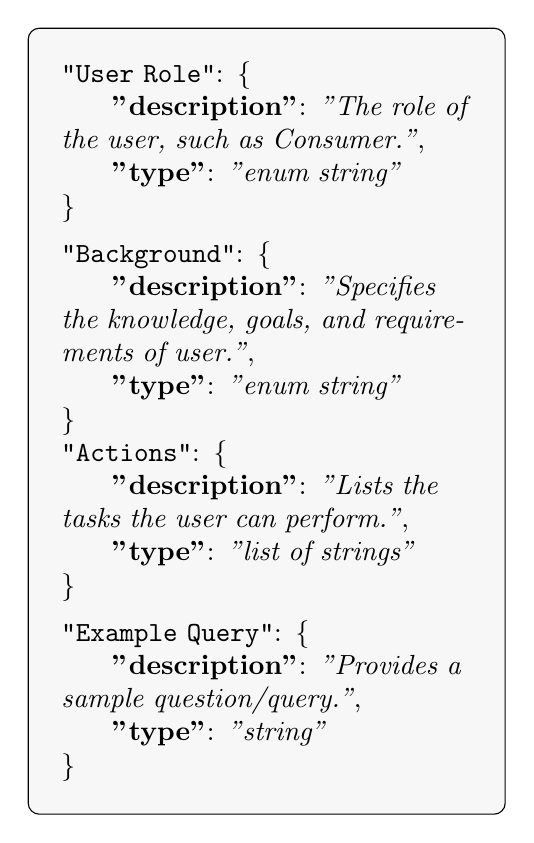
\begin{tikzpicture}
% Draw rounded rectangle with shadow
\node[rectangle, rounded corners, draw=black, fill=black!3!white, text width=0.43\textwidth, inner sep=12pt, align=left] (box) {
    \textbf{\texttt{"User Role"}}: \{\\
    \hspace{15pt} \textbf{"description"}: \textit{"The role of the user, such as Consumer."}, \\
    \hspace{15pt} \textbf{"type"}: \textit{"enum string"} \\
    \} \vspace{5pt}\\
    \textbf{\texttt{"Background"}}: \{\\
    \hspace{15pt} \textbf{"description"}: \textit{"Specifies the knowledge, goals, and requirements of user."}, \\
    \hspace{15pt} \textbf{"type"}: \textit{"enum string"} \\
    \} \\
    \textbf{\texttt{"Actions"}}: \{\\
    \hspace{15pt} \textbf{"description"}: \textit{"Lists the tasks the user can perform."}, \\
    \hspace{15pt} \textbf{"type"}: \textit{"list of strings"} \\
    \} \vspace{5pt}\\
    \textbf{\texttt{"Example Query"}}: \{\\
    \hspace{15pt} \textbf{"description"}: \textit{"Provides a sample question/query."}, \\
    \hspace{15pt} \textbf{"type"}: \textit{"string"} \\
    \}
};

\end{tikzpicture}
}
\caption{Use case specializations. For each use case, we define its role, goal, actions, and example query. For each property, we present its description and type.}
\label{fig:usecasedef}
\end{figure}

\begin{table*}[]
\centering
\caption{The actions and example query for each kind of user role defined for \chatiot.}
\label{tab:usecase}
\resizebox{\textwidth}{!}{

\begin{tabular}{p{1.5cm}|p{12cm}|p{4cm}}
%\begin{tabular}{@{}c@{\hskip 0.1cm}|
%    @{\hskip 0.1cm}>{\arraybackslash}p{10.5cm}@{\hskip 0.1cm}|
%    @{\hskip 0.1cm}>{\arraybackslash}p{5cm}@{\hskip 0.1cm}
%    }
\toprule
\toprule
\multicolumn{1}{c|}{Role} & \multicolumn{1}{c|}{Actions} & \multicolumn{1}{c}{Example Query}  \\ \midrule
Consumer  
& \romannumeral1) Assess the security of IoT devices before purchase or installation; \newline
\romannumeral2) Monitor ongoing security status and updates for existing devices;\newline
\romannumeral3) Make informed decisions based on security reports provided by \chatiot.
& Is it secure to use Signify Smart Lighting in home? \\
\midrule

Security Analyst  
&
\romannumeral1) Identify and evaluate security threats and vulnerabilities in IoT devices;\newline
\romannumeral2) Recommend mitigation strategies based on threat intelligence and analysis;\newline
\romannumeral3) Provide detailed security reports to stakeholders.
& Conduct a security assessment for TP-Link AX6000 Wi-Fi 6 Router. 
\\ \midrule

Technical Officer 
&
\romannumeral1) Ensure that IoT devices are deployed securely and operate within compliance guidelines;\newline
\romannumeral2) Oversee the application of security updates and patches;\newline
\romannumeral3) Monitor the security posture of the IoT ecosystem within their organization.
& Check the security labeling of the company's WiFi Routers,  including TP-Link, D-Link, and ASUS in Singapore. 
\\
\midrule

Developer
&
\romannumeral1) Design and develop secure IoT products by adhering to best practices and security standards;\newline
\romannumeral2) Continuously update products to address new vulnerabilities and threats;\newline
\romannumeral3) Provide accurate security documentation and updates to customers.
&
Develop a security enhancement roadmap for the next generation of TP-Link Wi-Fi routers.
\\
\midrule

Trainer 
&
\romannumeral1) Develop and deliver training programs on IoT security;\newline
\romannumeral2) Guide users and organizations on how to secure IoT devices and respond to incidents;\newline
\romannumeral3) Provide up-to-date information on IoT security trends and best practices.
&
Prepare a guide on the importance of cybersecurity labeling for smart locks like the August Smart Lock.
\\
\bottomrule
\bottomrule

\end{tabular}}
\end{table*}

In this section, we define five specialized use cases of \chatiot. 
Each use case is defined by \textit{four} fundamental properties: \textit{User Role}, \textit{Background}, \textit{Actions}, and \textit{Example Query}, within the IoT security domain.
The detailed specifications are illustrated in Figure~\ref{fig:usecasedef}.
The roles include \textit{Consumer}, \textit{Security Analyst}, \textit{Technical Officer}, \textit{Developer}, and \textit{Trainer}. 
Recall that we have discussed background in \S~\ref{sec:resgen}, we present the detailed actions and example query in the following context.


Table~\ref{tab:usecase} highlights the key actions associated with each user role, such as assessing the security of IoT devices, deploying security patches, or developing training programs on IoT security.
Additionally, it provides example queries for each role, demonstrating how \chatiot\ can be utilized to address the unique needs of various users. 
This structured approach ensures that \chatiot\ caters to a diverse range of users, offering tailored assistance and enhancing IoT security management across different scenarios.
Note that while we provide five use cases, they are not rigid or fixed. 
The use cases can be easily extended by defining new user roles, specifying the background (including knowledge, goals, and requirements), and outlining actions. Example queries can also be added to further clarify the context and functionality of each user role.

